Los asistentes inteligentes están buscando su hueco en todo hogar, y esto es un hecho.
Estos asistentes nos hacen la vida más sencilla, ayudando a actualizar y controlar toda la domótica de nuestras casas con acciones que hace unos años solo podíamos imaginarlas en películas de ciencia ficción.

El concepto de asistentes de voz, que tan de moda está ahora entre la población joven, junto con la gente de edad avanzada que necesita interacción en sus vidas puede ser una combinación perfecta para ayudarles a no perder el contacto con la sociedad.

La creación de un asistente que pueda resolver sus dudas, con el que puedan hablar, al que puedan preguntar a qué hora es la partida de cartas en el bar, o al que puedan pedir auxilio en caso de una caída, puede ser de gran utilidad para mejorar su día a día, al igual que servir de alivio para el resto de familiares que no pueden estar cerca de sus seres queridos, sabiendo que van a poder ser informados rápidamente de un posible accidente.

Pero el auge de los dispositivos asistentes pone en vilo la gestión de la privacidad e intimidad que hay dentro de nuestras casas,n y todo esto es debido a que pueden recolectar información a través de escuchar las conversaciones de nuestro día a día, siendo información que no sabemos a dónde va a parar, qué se va a hacer con ella.

Esta información es de un caracter sensible, ya que puede contener desde nuestros simples gustos, incluyendo nuestras necesidades, hasta nuestras tendencias políticas, siendo datos que pueden estar siendo utilizados por terceros, o incluso siendo vendidos ante nuestro desconocimiento.

La falta de soluciones en el mercado que cumplan todos estos puntos suponen una motivación para la creación de un asistente que no esté conectado constantemente a internet, ya que las personas de edad avanzada seguramente no tengan contratado el servicio, y que tampoco almacene datos de carácter sensible de los usuarios, sino que simplemente interaccione con cada persona, y la ayude en su día a día, tanto ofreciendo actividades de la misma localidad, como respondiendo cualquier pregunta que pase por la cabeza de quien lo posea, al igual que buscando ayuda en caso de que una persona requiera auxilio.

Antes de adentrar en la elección de un asistente inteligente, se expondrá qué es, y cuál es su funcionamiento, para entender mejor los motivos por los cuales se acaba eligiendo uno en vez de otro.

\subsubsection{Qué es un asistente inteligente}

Un asistente inteligente es simplemente una máquina programada de manera que su comportamiento se asemeje al de una persona a la que se solicita asistencia, como su propio nombre indica, pudiendo mantener una conversación que siga los protocolos de comunicación humana.

\begin{figure}[h!]
    \centering
    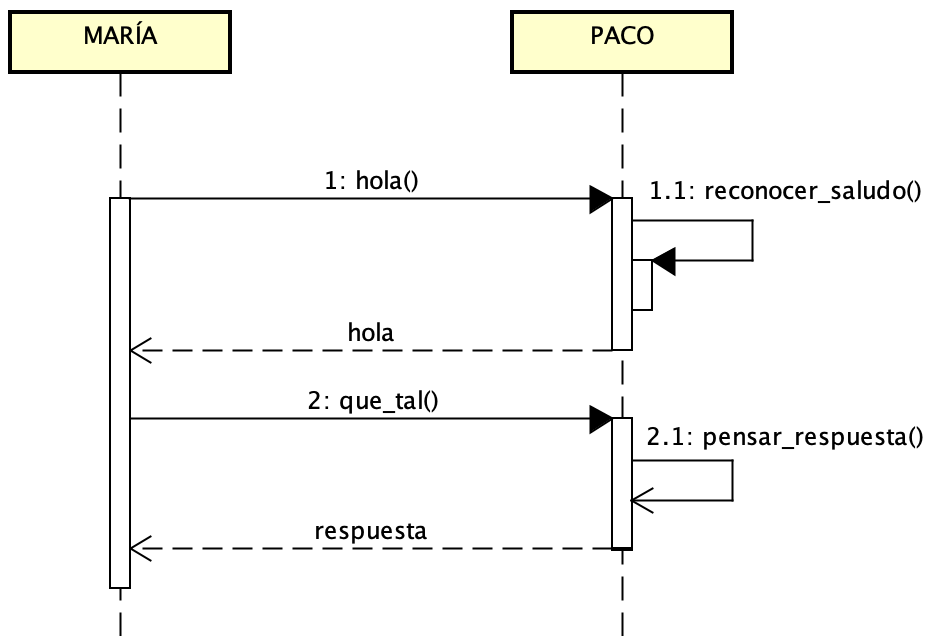
\includegraphics[width=10cm]{./img/sequence/human.png}
    \caption{Secuencia de comunicación humana}
    \label{fig:humanseq}
\end{figure}

Como se puede ver en la figura \ref{fig:humanseq}, un protocolo de comunicación entre dos personas se basaría en un saludo para entablar conversación, para posteriormente realizar una pregunta.

En el caso de los asistentes, el proceso de conversación se basa en lo mismo: un usuario saluda al asistente mediante el uso de una palabra o conjunto de palabras, al que se llamará \textbf{hotword}, que cuando sea reconocido por el asistente inteligente, devolverá el saludo.
Es entonces cuando el usuario debe realizar la pregunta o solicitar la información que requiera.
Una vez hecha la pregunta, el dispositivo se pondrá a pensar la posible respuesta, entrando en el proceso al que se llamará \textbf{reconocimiento de los hechos}. Una vez identificados los hechos, devolverá la respuesta que más se acerque a lo deseado, gracias a un entrenamiento previo.

\subsubsection{Cómo piensa el asistente}

El proceso de pensamiento analizado entre los principales asistentes, que se expondrá en este capítulo tiene una estructura similiar independientemente del tipo de asistente que se trate, asemejándose a la figura \ref{fig:humasseq}.

\begin{figure}[h!]
    \centering
    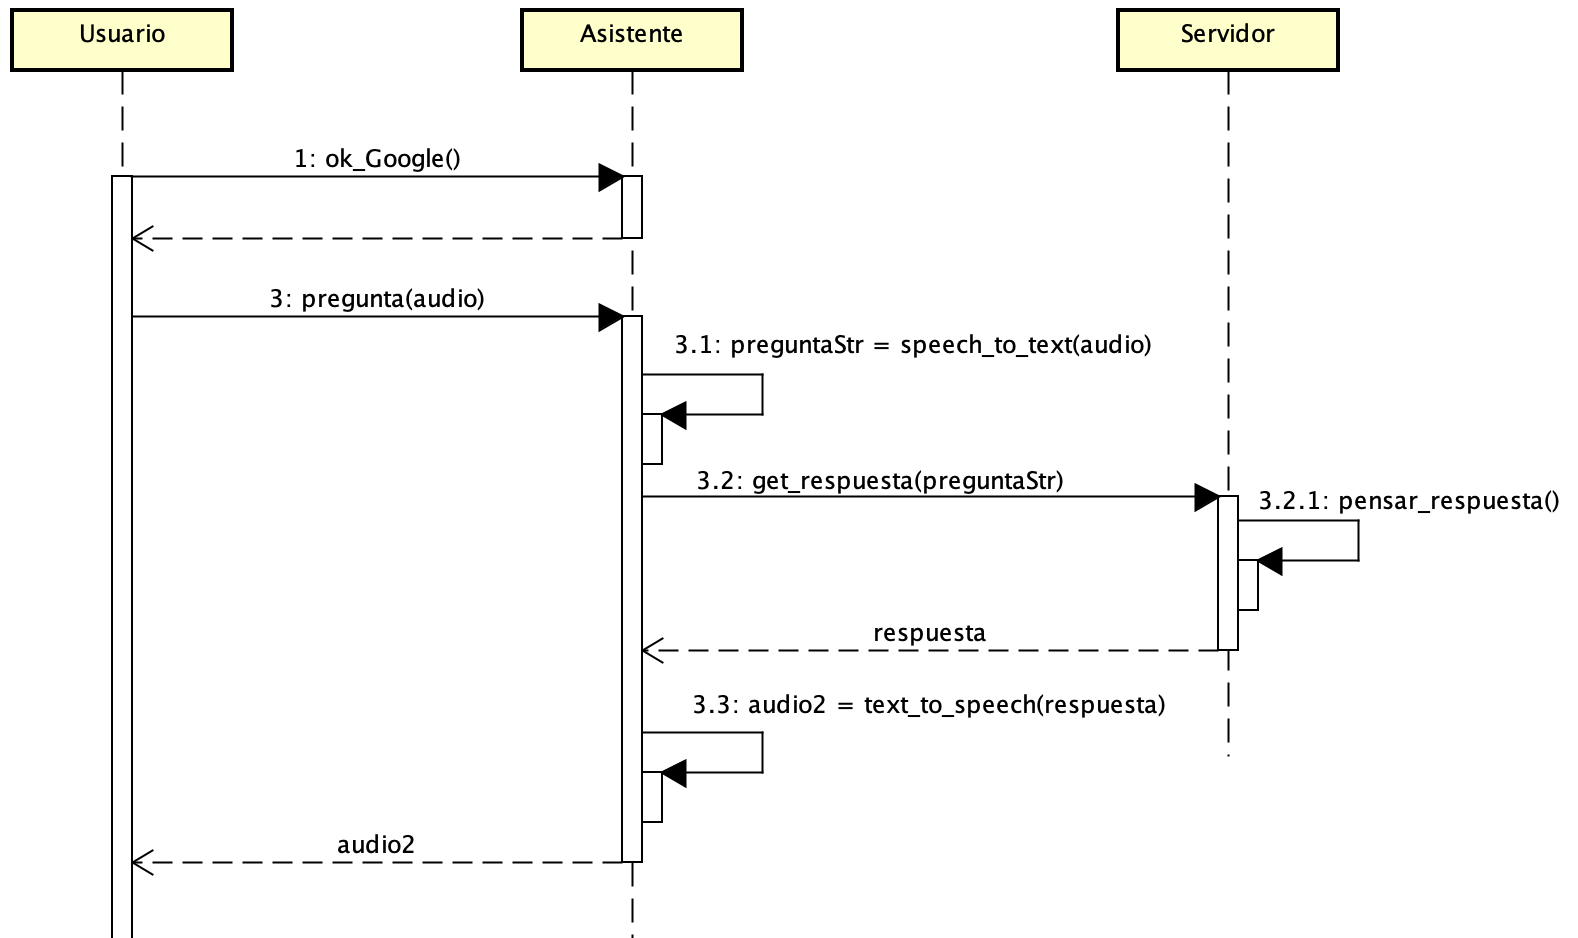
\includegraphics[width=14cm]{./img/sequence/humasseq.png}
    \caption{Secuencia de comunicación humano-asistente}
    \label{fig:humasseq}
\end{figure}

Lo que diferencia a un asistente de otro, es la manera en la cual piensa la respuesta, dando mayor validez a un asistente que dé una respuesta más aproximada a lo solicitado.
Para esto, la mayoría de asistentes tienen el procesamiento de la respuesta en la nube debido a la gran cantidad de información que tienen almacenada para contrastar los hechos capturados, al igual que también tienen en la nube el proceso de speech-to-text o el de text-to-speech.
